\documentclass[11pt]{article}

% \usepackage[style=authoryear,natbib=true]{biblatex}
\usepackage[numbers,sort&compress]{natbib}  
%% Daniel added this, should help citations look nicer. You may need to delete temp files and rebuild the latex document from a clean start.

\newcommand{\daniel}[1]{{\textbf{{\small{\color{magenta}DL}: #1{\color{magenta}$\circ$}}}}} 
\newcommand{\owen}[1]{\textbf{{\small{\color{red}OK}: #1{\color{red}$\circ$}}}} 
\newcommand{\ed}[1]{\textbf{{\small{\color{blue}ED}: #1{\color{blue}$\circ$}}}}

%\renewcommand{\daniel}[1]{}
%\renewcommand{\owen}[1]{}
%\renewcommand{\ed}[1]{}

% Use utf-8 encoding for foreign characters
\usepackage[utf8]{inputenc}
\usepackage{url}
% Setup for fullpage use
\usepackage{fullpage}
\usepackage{color}
\usepackage{subfig}
\usepackage{hyperref}
\usepackage{algorithm2e} % \usepackage[noend]{algorithm2e}
\usepackage{algorithmic}

% Uncomment some of the following if you use the features
%
% Running Headers and footers
%\usepackage{fancyhdr}

% Multipart figures
%\usepackage{subfigure}

% More symbols
%\usepackage{amsmath}
%\usepackage{amssymb}
%\usepackage{latexsym}

% Surround parts of graphics with box
\usepackage{boxedminipage}

% Package for including code in the document
\usepackage{listings}

% If you want to generate a toc for each chapter (use with book)
\usepackage{minitoc}

% This is now the recommended way for checking for PDFLaTeX:
\usepackage{ifpdf}

%\newif\ifpdf
%\ifx\pdfoutput\undefined
%\pdffalse % we are not running PDFLaTeX
%\else
%\pdfoutput=1 % we are running PDFLaTeX
%\pdftrue
%\fi

% \ifpdf
\usepackage[pdftex]{graphicx}
% \else
% \usepackage{graphicx}
% \fi

\title{RMS and Backpropagation for Feedforward Neural Networks}
\author{Eduardo Gutarra}

% \date{2010--06--13}

\begin{document}
	
\ifpdf
\DeclareGraphicsExtensions{.pdf, .jpg, .tif}
\else
\DeclareGraphicsExtensions{.eps, .jpg}
\fi
	
\maketitle
	
\section{Introduction} % (fold)
\label{sec:introduction}

Artificial neural networks are computational models that mimic the architecture, structure and/or functional aspects of biological
neural networks such as the human brain. They are comprised of multiple processing elements called neurons which are interconnected
through links. Often, these links have weights associated to them called synaptic weights. These weights scale the signals received from
different neurons, allowing the network to process patterns and generate an output pattern. The synaptic weights are free parameters
that may be changed, allowing the neural network to change its behavior. In artificial neural networks, neurons are often grouped
together in layers or slabs and a neural network may be composed of 1 or more of these~\cite{skapura}. As an example, a feedforward
neural network is illustrated in Figure~\ref{fig:figures_ffwdnn}.

The entire behavior of the neural network is determined by the individual behaviors of neurons that comprise it. Each neuron gathers
input from the external environment or other neurons. The neuron then generate a signal that may be input to other neurons or the final
output. This process continues throughout the network until a response is produced on the external environment. Neurons modulate and
aggregate the input to calculate an activation value. The activation value may be the same or it could be a function of the aggregation.
The activation value then is passed as a parameter to an activation function, which determines the output of the neuron (See Figure~\ref{fig:figures_single_neuron}).

Neural networks possess important advantages and capabilities as computational models. Among these include their ability to: solve
problems of nonlinear nature, perform input-output mapping through a learning process, adaptation to new situations, and their inherent
parallelism~\cite{Haykin:1994:NNC:541500}. One of the greatest advantages of using a neural network is that we do not program it with a
configuration to solve a problem. It is actually programmed to learn and adapt to solve a problem. Neural networks have two types of
learning supervised and unsupervised learning. Supervised learning consists in giving a network a set of points and allowing to correct
its prediction by giving it the expected output. Unsupervised learning is often used when the network cannot be provided with a target
output, and therefore works with evolutionary models. We focus on supervised learning for this report.

Even though biological neurons are 6 orders of magnitude slower than the integrated circuits found in today's computer processors. They
work as a massively parallel system allowing efficient solutions to complex problems such as facial recognition. These problems are
still a challenge today for today's artificial neural networks, and other computational models. Artificial neural networks have been
successfully applied in applications such as: Function approximation or regression analysis and Classification, including pattern and
sequence recognition among others.

Our interest in this report is confined to a class of neural networks which emulate the process of learning. This report examines two
different algorithms for training feedforward neural networks. One algorithm is the Back-propagation algorithm and the other is the Root
Mean Square (RMS) Minimization algorithm.

\begin{figure}[]
	\centering
		\subfloat[\label{fig:figures_ffwdnn} A feedforward neural network with labeled constituents]{	
				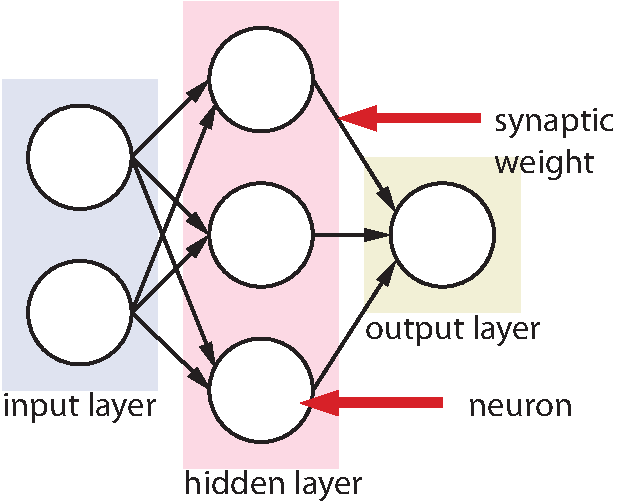
\includegraphics[height=0.30\columnwidth]{figures/ffwdnn.pdf}
		}
		\hspace{2mm} 
		\subfloat[\label{fig:figures_single_neuron} A neuron $j$ with input $x_{k}$ from with synaptic weight $w_{jk}$. The neuron integrates the inputs modulated by their respective weights, and calculates an output with activation function $f$]{	
				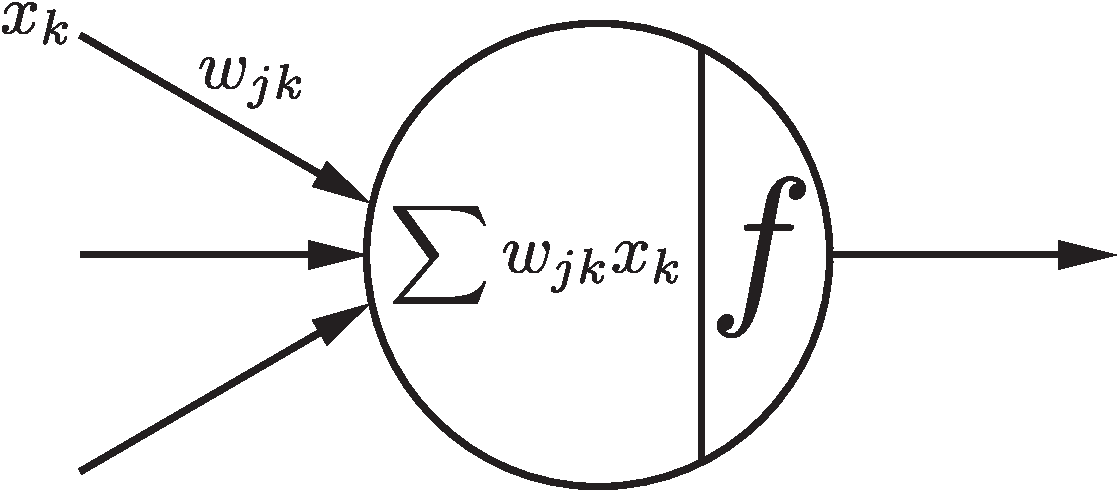
\includegraphics[height=0.20\columnwidth]{figures/single_neuron.pdf}
		}
		\caption{A feedforward neural network and a magnified view of its processing element the neuron}
	\label{fig:figures_ffwdnn_Neuron}	
\end{figure}

\section{Feedforward Neural Networks} % (fold)
\label{sec:feedforward_neural_networks}

In a feedforward neural network only neurons of adjacent layers are interconnected with synaptic weights. Each layer of the neural
network has connections to the next layer and there are no connections oriented backwards. The feedforward neural network begins with an
input layer which may be connected to a hidden layer or directly to an output layer. The first layer is the input layer. It connects
directly to the external environment and captures the input patterns presented to the network. The last layer is the output layer which
produces the output pattern to the external environment. All other layers are considered hidden and may or may not be present.

The processing of a feedforward neural network begins when an external pattern made is copied to the input layer. The neurons of the
input layer communicate the pattern to the following layers through synapses. The pattern is then received by neurons of non-input
layers and modulated by the weight of their connections. We denote weights as $W_{jk}$, where $j$ is the neighbor neuron, and $k$ is the
neuron . Each neuron receives stimulation from other neurons, except the input layer which captures the pattern. Once the inputs are
modulated, they are integrated and an activation value is determined. Often the activation value is just the integration of the
modulated inputs, but may also be a function $F_{i}(a_{i}(t-1), net_{i}(t))$, where $a_{i}(t-1)$ is the activation at the previous time
step and $net_{i}(t)$ is the integration of modulated inputs. (see Algorithm~\ref{alg:feedforward}
)

\begin{algorithm}% [H]
\dontprintsemicolon
\KwIn{Set of inputs from the environment}
\KwOut{Set of output values calculated by the feedforward neural network}
\SetLine
\ForEach{layer from the first non-input layer to the output,}
{
	\ForEach{unit on the current layer,}
	{
		Set the accumulated input value for this unit to zero\;
			\ForEach{ input connection to this unit,} 
			{
				Compute the modulated input across this connection\;
				Add the modulated input to the accumulated input\;
			}
		Convert the accumulated input to its corresponding output\;
		Store the output value for the unit in the layer structure\;
	}
	Return the output values from the top-most layer structure\;
}

\caption{The Feedforward Algorithm (Taken from~\cite{skapura})}
\label{alg:feedforward}
\end{algorithm}

% section feedforward_neural_networks (end)

% section introduction (end)

\section{Data Structure and Algorithms} % (fold)
\label{sec:data_structure_and_algorithms}

To work with the neural network, we represent it using a data structure that is used by the learning algorithms to store the information
relevant to neurons and layers. We examine two different algorithms to train the feedforward neural network. One algorithm is the
Back-propagation algorithm and the other is the Root Mean Square (RMS) Minimization algorithm.

\subsection{Data Structure} % (fold)
\label{sub:data_structure}

We do not have to implement neural networks to study them, it is possible to simulate their execution to solve problems in a computer.
We build data structures in order to represent the neural network. A neural network can be thought of as a directed graph, where the
neurons are nodes, and the synaptic weights are the arcs of the graph. Because we focus on feed-forward networks, our graphs can further
be specified as directed acyclic graphs. These graphs do not require a full matrix to represent all possible connections between the
neurons. Instead we use an array of matrices where each matrix stores the synaptic weights of the departing connections from the current
neuron in the current layer to the neurons of the next layer (see Figures~\ref{fig:figures_ffwdnn2} and
\ref{fig:figures_DataStructure1}).

We may also add an additional free parameter that does not link to other neuron, and has a constant input. We call this parameter the
bias, and it allows the activation functions to translate along the y-axis. We include the bias as one more row of elements in each
weight matrix that represents connections between neurons (see Figures~\ref{fig:figures_ffwdnn3} and \ref{fig:figures_DataStructure2}).

\begin{figure}[]
	\centering
		\subfloat[\label{fig:figures_ffwdnn2}]{	
				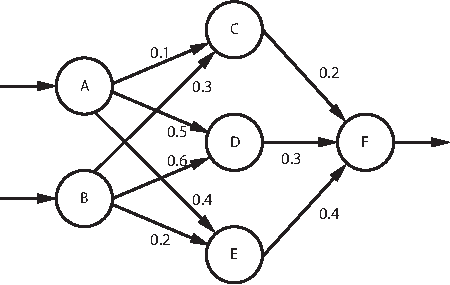
\includegraphics[width=0.45\columnwidth]{figures/ffwdnn2.pdf}
		}
		\hspace{2mm}
		\subfloat[\label{fig:figures_ffwdnn3}]{	
				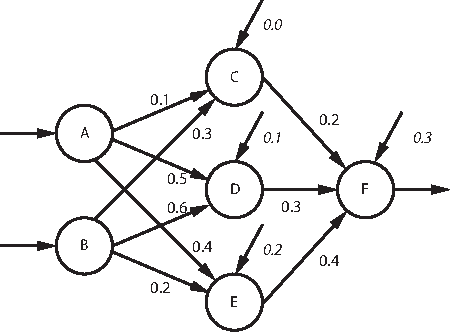
\includegraphics[width=0.45\columnwidth]{figures/ffwdnn3.pdf}
		}

		\subfloat[\label{fig:figures_DataStructure1}]{	
				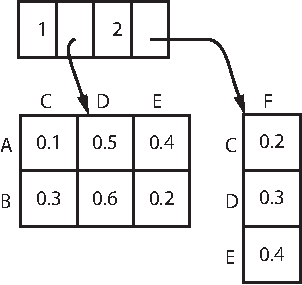
\includegraphics[width=0.35\columnwidth]{figures/DataStructure1.pdf}
		}
		\hspace{8mm} 
		\subfloat[\label{fig:figures_DataStructure2}]{	
				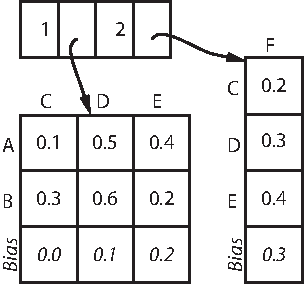
\includegraphics[width=0.35\columnwidth]{figures/DataStructure2.pdf}
		}
		\caption{Feedforward neural networks (a and b) with their corresponding computer representation (c and d). Figures~\ref{fig:figures_ffwdnn2} and \ref{fig:figures_DataStructure1} represent a neural network without bias parameters. Figures~\ref{fig:figures_ffwdnn3} and \ref{fig:figures_DataStructure2} represent a neural network with bias parameters}
	\label{fig:figures_ffwdnn_DS}	
\end{figure}

% subsection data_structure (end)

\subsection{Backpropagation training algorithm} % (fold)
\label{sub:backpropagation_training_algorithm}

Back-propagation is a method of supervised learning. It is used to train our feedforward neural network. To use the back-propagation
algorithm we provide it with both example inputs and target outputs. The outputs generated by the neural network are then compared
against the target outputs of the given example. Using the target outputs, the back-propagation training algorithm then calculates
errors and adjusts the weights of the various layers backwards from the output layer to the input layer. The degree of adjustment in the
weights and bias can be scaled. The scaling factor used is called the learning rate $\eta$, and it determines how quickly the neural
network attempts to learn a mapping of input to output.

Back-propagation is often used to train feedforward neural networks but it can also be used to train other types of networks, and
likewise feedforward networks may be trained with other methods. In this report, we only examine back-propagation when it is used to
train a feedforward neural network. Algorithm~\ref{alg:backpropagation} illustrates the process in further detail.

\begin{algorithm}% [H]
\dontprintsemicolon
\KwIn{Set of examples $E$}
\tcc{$e$ is a single example} 
\tcc{$I(e)$ set of inputs in a single example}
\tcc{$T(e)$ set of target outputs for a given example}
\tcc{$O(e)$ are the target outputs of the example}
\tcc{Each iteration of this loop we an epoch}

% \KwOut{Set of output values calculated by the feedforward neural network}
\SetLine
\ForEach{ example $e$ in a set of examples $E$}
{
	Calculate $O(e)$ for $I(e)$ with feedforward (refer to Algorithm~\ref{alg:feedforward})\;
	Call function \textbf{CalculateOutputDeltas}($O(e)$, $T(e)$)\;
	Call function \textbf{CalculateInternalDeltas}\;
	Call function \textbf{UpdateWeights}\;
}

\textbf{CalculateOutputDeltas($O(e)$, $T(e)$):}

Get output values $O(e)$ from the output layer neurons\;
\ForEach{ individual output value $O(e)_i$ }
{
	Calculate error $\epsilon$ as $O(e)_i$ - $T(e)_i$\;
	Calculate \textbf{$\delta_{O(e)_{i}} = \partial{f(O(e)_{i})}  \times \epsilon $}\;
	Add $\delta_{O(e)_{i}}$ to set of deltas $\Lambda$
}  

\textbf{CalculateInternalDeltas:}

Let $\Lambda_{i+1}$ be the next layer's set of deltas\;
\ForEach{ non-output layer $i$ from the penultimate to the first}
{
	\ForEach{ neuron $j$ in this layer } 
	{
	Initialize error $\epsilon$ as $0.0$\;
		\ForEach{ neuron $k$ of the next layer} 
		{
			Calculate $\epsilon$ as $\epsilon + \Lambda_{i+1,k} W_{ijk}$\;
		}
		$\Lambda_{i,j} = \partial{f( \epsilon \times \mbox{neuron } j\mbox{'s output} )}$\;
	}
} 

\textbf{UpdateWeights:}

\tcc{$\eta$ is the learning rate}
\ForEach{ layer $i$ }
{
	\ForEach{ neuron $j$ in this layer } 
	{
		\ForEach{ neuron $k$ of the next layer} 
		{
			Calculate $\Delta W_{ijk}$ as $\Lambda_{i,j} \times \mbox{neuron } j\mbox{'s output}$\;
			$W_{ijk} \leftarrow \eta \times \Delta{W_{ijk}}   $\;
		}
	}
} 

\caption{The Back-propagation Algorithm }
\label{alg:backpropagation}
\end{algorithm}

\begin{figure}[]
	\centering
		\subfloat[\label{fig:figures_backpgtn1}]{	
				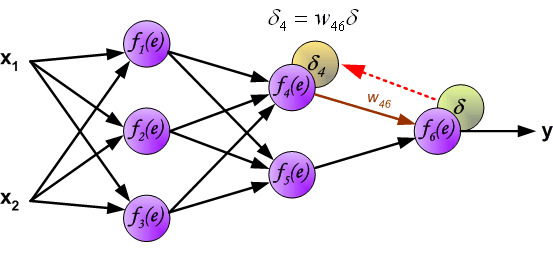
\includegraphics[width=0.49\columnwidth]{figures/backpgtn1.png}
		}
		\subfloat[\label{fig:figures_backpgtn2}]{	
				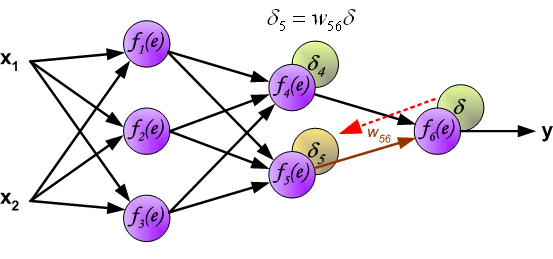
\includegraphics[width=0.49\columnwidth]{figures/backpgtn2.png}
		}
		
		\subfloat[\label{fig:figures_backpgtn3}]{	
				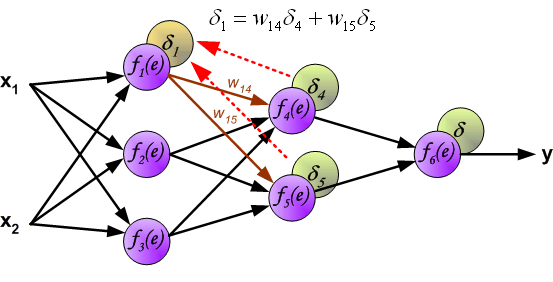
\includegraphics[width=0.49\columnwidth]{figures/backpgtn3.png}
		}
		\subfloat[\label{fig:figures_backpgtn4}]{	
				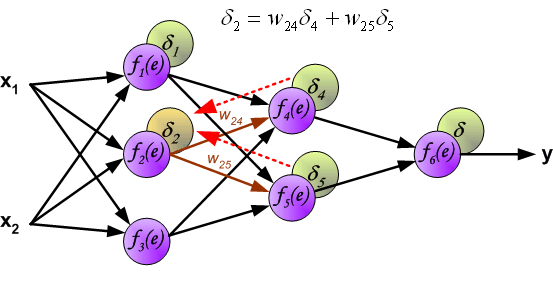
\includegraphics[width=0.49\columnwidth]{figures/backpgtn4.png}
		}
		
		\subfloat[\label{fig:figures_backpgtn5}]{	
				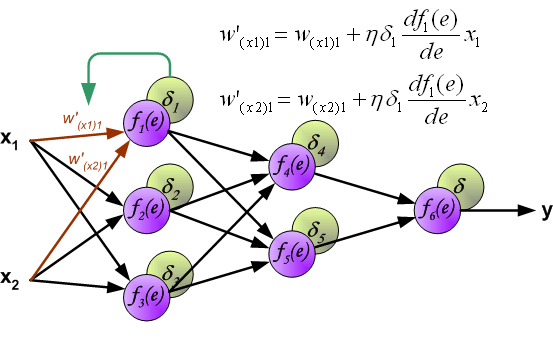
\includegraphics[width=0.49\columnwidth]{figures/backpgtn5.png}
		}
		\subfloat[\label{fig:figures_backpgtn6}]{	
				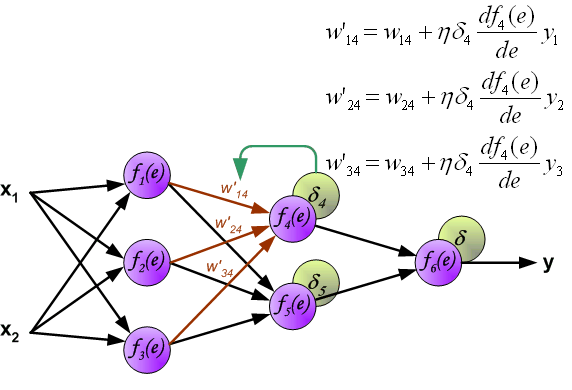
\includegraphics[width=0.49\columnwidth]{figures/backpgtn6.png}
		}
		
		\caption{An illustration of the Back-propagation algorithm. (Taken from \cite{vlsibackp_t})}
	\label{fig:figures_backpgtn}	
\end{figure}

% subsection backpropagation_training_algorithm (end)

\subsection{RMS Minimization Algorithm} % (fold)
\label{sub:rms_minimization_algorithm}

Another algorithm we use to train the feedforward neural network is the Root Mean Square (RMS) Minimization algorithm. For this
algorithm we also provide example inputs and target outputs. We run the feedforward algorithm with each individual example generating
the corresponding outputs of the neural network. After generating the outputs we calculate the root mean square between outputs given by
the neural network and target output provided by the example. We keep this calculation as $\mbox{RMS}_{\mbox{old}}$.

Next, a small change is made to one of the weights of the neural network, and the feedforward algorithm is called again to calculate new
outputs for the neural network. We again, take the root mean square between outputs and targets which we call $\mbox{RMS}_{\mbox{new}}$.
We then calculate a slope by taking the difference between $\mbox{RMS}_{\mbox{old}}$ and $\mbox{RMS}_{\mbox{new}}$, and divide by the
change made to the weight. We use this slope to determine what change needs to be made to improve the RMS between the output of our
network and the target from the example. Unlike the back-propagation method, this method performs a $\mbox{num}(E)$ feedforward passes,
where $\mbox{num}(E)$ is the number of examples used to train the network. The process is illustrated in further detail in
Algorithm~\ref{alg:RMSminimization}.

\begin{algorithm}% [H]
\dontprintsemicolon
\KwIn{Set of examples $E$, constants $\alpha$ and $\epsilon$}
\tcc{We call each iteration of this loop an epoch}
Set $\Delta W$ to $0.01$\;
\SetLine
\ForEach{layer $i$ from the first non-input layer to the output,}
{
	\ForEach{layer $i$ from the first non-input layer to the output,}
	{
		\ForEach{neuron $j$ on the current layer,}
		{
				\ForEach{ connection $k$ to a neuron of the next layer,} 
				{
					Calculate $\mbox{RMS}_{\mbox{o}}$ as \textbf{CalculateRMS}($E$)\;
					Set $W_{ijk}$ to $W_{ijk}$ + $\Delta W$\;
					Calculate $\mbox{RMS}_{\mbox{n}}$ as \textbf{CalculateRMS}($E$)\;
				
					Calculate $\Delta RMS$ as $ \frac{\mbox{RMS}_{\mbox{n}}-\mbox{RMS}_{\mbox{o}}}{\Delta W} $\;
				
					\If{ $\Delta RMS \neq 0.0 $}{
					  Calculate $\Delta W_{ijk}$ as $\alpha \times \Delta W_{ijk} - \epsilon \times \Delta RMS$\;
					  Calculate $W_{ijk}$ as $W_{ijk} + \Delta W_{ijk}$\;
					}
				}
		}
	}
}

\textbf{CalculateRMS($E$)}:
\dontprintsemicolon
\tcc{$e$ is a single example} 
\tcc{$I(e)$ set of inputs in a single example}
\tcc{$T(e)$ set of target outputs for a given example}
\tcc{$O(e)$ are the target outputs of the example}
Set $\epsilon$ to $0.0$\;
\ForEach{example $e$ in the set of examples $E$} 
{
	$O(e)$ $\leftarrow$  Call feedforward algorithm with $I(e)$ (see Algorithm~\ref{alg:feedforward})\;
	\ForEach{ output $O(e)_i$ obtained from the neural network }
	{
		Calculate $\epsilon$ as $\epsilon + (O(e)_{i} - T(e)_{i})^{2}$\;
	} 
	
}
\Return $\frac{\epsilon}{\mbox{num}(E) - 1}$ \tcc*{ $\mbox{num}(E)$ is the total number of examples in $E$}
\vspace{5mm}
\caption{The RMS Minimization Algorithm}
\label{alg:RMSminimization}
\end{algorithm}


% subsection rms_minimization_algorithm (end)

% section data_structures_and_algorithms (end)

\section{Experiments and Results} % (fold)
\label{sec:results}

A set of system experiments are performed where we test the RMS and back-propagation training methods. We compare the time complexity
between both training methods as well as their accuracy after training is completed. The set of examples to train the network are
generated by taking two numerical inputs and adding them to generate the expected output. This data is normalized so that its range is
between -1 and 1. The feedforward neural network is configured with $2$ neurons in the input layer, $3$ in the middle layer and $1$ in
the output layer. The neurons in the middle layer use a hyperbolic tangent activation function, and the neurons in the output layer use
a linear function. In our procedures we change different parameters of the neural network, and observe the behavior in time complexity
and accuracy.

\subsection{Time Complexity} % (fold)
\label{sub:time_complexity}

We tested the time complexity of both algorithms in different aspects that may be configured in the neural network. We look at time as
we vary the number of neurons in the middle layer, the number of iterations, and the number of points in the example. Experimentally, we
notice that both algorithms exhibit linear growth in time when we change the number of iterations or examples (see
Figures~\ref{fig:docs_graphs_TimeItrns} and \ref{fig:docs_graphs_TimeSmpls}). The algorithms however differ in that RMS Minimization
grows quadratically whereas back-propagation grows linearly when the number of neurons in the middle layer is varied (see
Figure~\ref{fig:docs_graphs_TimeNrns}). Finally, in all our system experiments, back-propagation was faster than RMS Minimization.

To look at the time complexity analytically we estimate the number of operations made by both algorithms. The number of operations is
proportional to the number of weights and biases in the neural network in many stages of the different algorithms. The number of weights
between two layers of neurons is the product between the total number of neurons in two adjacent layers. Therefore the total number of
weights for the entire network is $\sum_{i=1}^{n}N_{i-1}N_{i}$ where $N_{i}$ is the number of neurons in each layer, and $n$ is the
total number of layers. For the back-propagation algorithm, the number of operations in a single epoch depends on the number of weights
and biases. To account for the biases we count one bias for each neuron that is not in the input layer. Therefore the total number of
biases is $\sum_{i=1}^{n}N_{i}$. We denote the total number of connections including weights and biases as
$c=\sum_{i=1}^{n}N_{i-1}N_{i} + \sum_{i=1}^{n}N_{i}$.

For each iteration of the back-propagation algorithm we run the feedforward algorithm for every example in the set of examples $E$. The
feedforward algorithm has a number of operations that is proportional to the number of connections in the neural network, which we
denote as $c$. After the neural network outputs are generated, the algorithm proceeds to calculate an error between expected output and
input with the \textbf{CalculateOutputDeltas} procedure. The number of operations in this method is proportional to the number of
outputs of the neural network denoted $o$. The error is propagated backwards throughout the rest of the network with the
\textbf{CalculateInternalDeltas} method. The number of operations made in this method is proportional to the number of deltas that we
need to adjust the connections of the neural network. The number of deltas we must save is equal to the number of neurons that are in
the output layer and middle layers which is also equal to the number of biases we keep. Therefore the number of operations in
\textbf{CalculateInternalDeltas} is proportional to $\sum_{i=1}^{n}N_{i}$. Finally in the \textbf{UpdateWeights} method, the weights are
adjusted with the deltas that were calculated in the \textbf{CalculateInternalDeltas} and \textbf{CalculateOutputDeltas} methods.
Because the the adjustments are done for every weight and bias, the total number of operations in this last method is proportial to the
number of connections. The analysis for back-propagation is summarized in Table~\ref{tab:backpropagation}.

\begin{table}
	\begin{center}
		\begin{tabular}{ccc}
		\hline
		& Calls & Estimated \# of ops.\\
		\hline
		Feedforward & $\mbox{num}(E)i$ & $\propto c$\\
		CalculateOutputDeltas & $\mbox{num}(E)i$ & $\propto o$\\
		CalculateInternalDeltas & $\mbox{num}(E)i$ & $\propto b$\\
		UpdateWeights & $\mbox{num}(E)i$ & $\propto c$\\
		\hline
		Total & & $\mbox{num}(E)i(2c+o+b)$\\
		\hline
		\end{tabular}
		\caption{Estimated number of operations performed at each stage of the Back-propagation algorithm. Here, $c$ is the number of connections, $i$ is the number iterations, $o$ is the number of outputs, and $\mbox{num}(E)$ is the number of examples.}
	\end{center}
	\label{tab:backpropagation}
\end{table}

\begin{table}
	\begin{center}
		\begin{tabular}{ccc}
		\hline
		 & Calls & Estimated \# of ops.\\
		\hline
		CalculateRMS & $2ci$ & $\propto \mbox{num}(E)$\\
		Feedforward called by CalculateRMS & $\mbox{num}(E)$ & $\propto c$\\
		\hline
		Total &  & $2c^2\mbox{num}(E)i$\\
		\hline
		\end{tabular}	
	\end{center}
	\caption{Estimated number of operations performed at each stage of the RMS minimization algorithm. Here, $c$ is the number of connections, $i$ is the number iterations, and $\mbox{num}(E)$ is the number of examples.}
	\label{tab:RMSminimization}
\end{table}

In each iteration of the RMS Minimization algorithm the method \textbf{CalculateRMS} is calculated twice for every connection. The two
calculations are made to determine the weight or bias adjustment necessary to improve the error between the neural network's output and
the expected output provided in the examples. The method \textbf{CalculateRMS} has a number of operations proportional to the number of
examples in the set of examples. To calculate the output generated by the neural network the feedforward algorithm is called by the
\textbf{CalculateRMS}. The feedforward algorithm is called by \textbf{CalculaterRMS} for every example in the set of examples. The
number of operations performed in the feedforward algorithms is proportional to the number of connections. RMS Minimization exhibits
linear growth to variations of all aspects of the neural network, but those related to the number of connections in the neural network.
This means that when the number of neurons is modified in the neural network, it exhibits quadratic growth in time. The analysis for RMS
minimization is summarized in Table~\ref{tab:RMSminimization}.

For the RMS algorithm the number of operations in a single epoch depends on both the number of weights and the number of is squared
because we run the feedforward algorithm for each change we do on a single weight.

\begin{figure}[]
	\centering
		\subfloat[\label{fig:docs_graphs_TimeNrns}]{	
				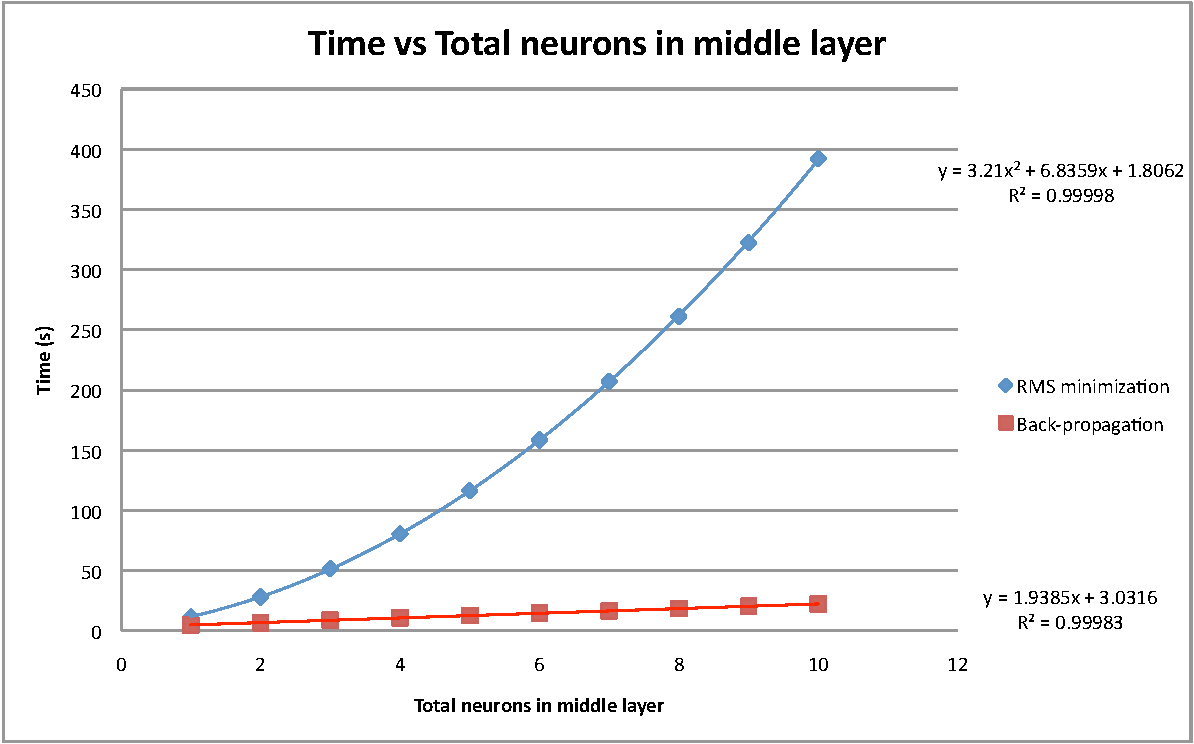
\includegraphics[width=0.60\columnwidth]{../docs/graphs/TimeNrns.pdf}
		}                                           
		   
		\subfloat[\label{fig:docs_graphs_TimeItrns}]{  
				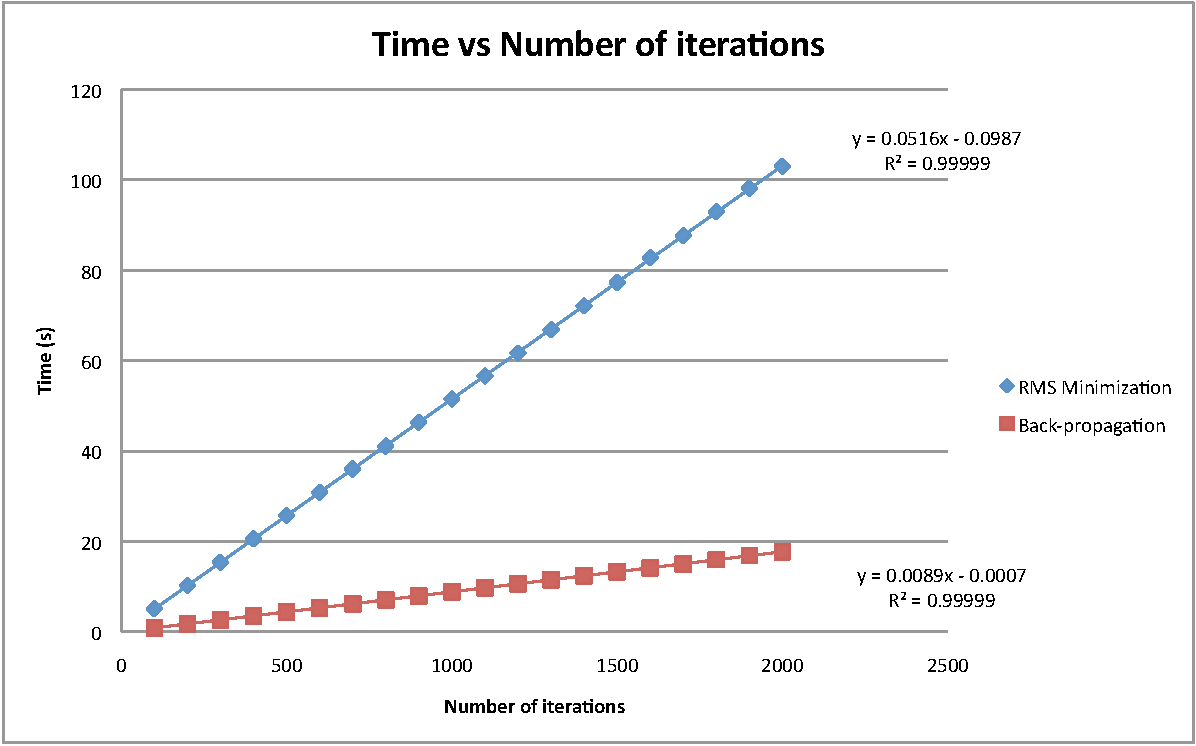
\includegraphics[width=0.60\columnwidth]{../docs/graphs/TimeItrns.pdf}
		}
		
		\subfloat[\label{fig:docs_graphs_TimeSmpls}]{  
				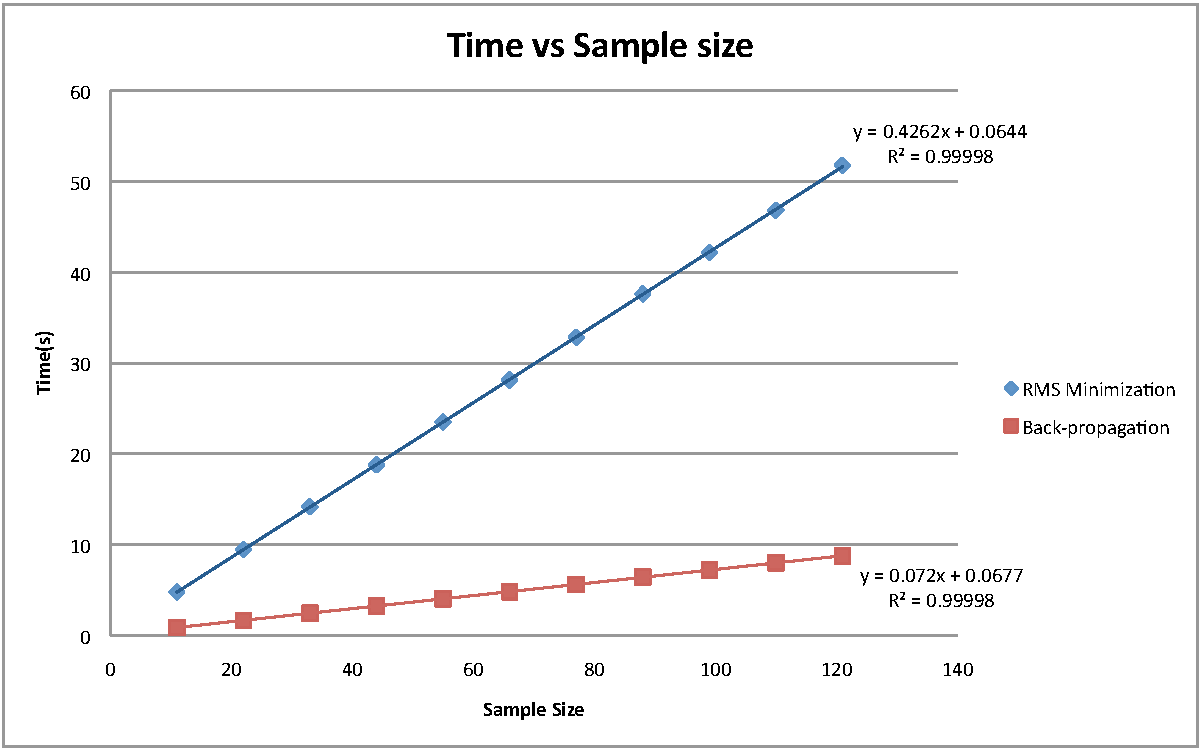
\includegraphics[width=0.60\columnwidth]{../docs/graphs/TimeSmpls.pdf}
		}
		\caption{Comparison in times between back-propagation and RMS minimization training algorithms. In Figure~\ref{fig:docs_graphs_TimeNrns} the the number of neurons in the middle layer is varied and time is measured. In Figure~\ref{fig:docs_graphs_TimeItrns} the number of iterations is varied. In Figure~\ref{fig:docs_graphs_TimeSmpls} the size of the sample is varied }
	\label{fig:docs_graphs_Time}	
\end{figure}

% subsection time_complexity (end)

\subsection{Training Accuracy} % (fold)
\label{sub:training_accuracy}

Here we will talk about the difference in training accuracy between the backpropagation and RMS minimization algorithms.

% subsection training_accuracy (end)

\subsection{A more Complex Problem} % (fold)
\label{sub:a_more_complex_problem}

To test the network we chose a more complicated problem. The problem consists in predicting the behavior of a mass attached to the end
of a spring that is connected to a fixed object. Ideally without the effect of friction and other \textbf{phenomena}, the system becomes
an harmonic oscillator. However if we add a damper ... \textbf{I need help here}. To simulate this physical phenomenon we used the
following equation:
\begin{eqnarray}\label{eqn:damping}
	x(t) = Ae^{-\alpha t}\cos{\beta t+\phi}.
\end{eqnarray}
Here, the position $x$ is determined by the amplitude $A$, the time $t$, and the constants $\alpha$ and $\beta$. Using this formula we
calculate the position of the mass, for a given time. We chose an amplitude $A=1$, and set the constants $\alpha$ and $\beta$ to $-3$
and $20$ respectively. We let $\phi=0$ for the first experiments, where we test the network on the same data it has learned.

Because we want the neural network to learn the behavior of this curve, we feed it the following $2$ inputs: The position in the
previous time step $x(t-1)$, and the position for the current time step $x(t)$. As the target output we have the position of the mass in
the next time step, $x(t+1)$.

We configured the neural network with $2$ neurons in the input layer, $3$ in the middle layer and $1$ in the output layer. The
hyperbolic tangent function was used as the activation function for the neurons in the middle layer, and for the output neuron a linear
activation function was used. The feedforward neural network was trained on $100$ sample points for $40000$ iterations with a learning
rate of $0.25$ using the back-propagation algorithm.

The weights of the neural network were initialized randomly. The neural network was trained using $10$ different randomized sets of
weights. The weights for the neural network producing the least error with the target output were saved. The different training sessions
are summarized in Table~\ref{tab:training_seeds}. The training sessions are sorted from best configuration being seed $9$, to worst,
seed $0$. The change in error for each iteration in the training session seeds $9$ and $0$ is illustrated in
Figure~\ref{fig:bpgt-3.0_damping_test_Trainings}. Logarithmic scale is used for this plot because the error descends dramatically in the
first iterations and slows down for later iterations. We observed that seed $0$ reaches a minimum in an earlier iteration than seed $9$.
Conclusively one can observe that some initial configurations will reach a local minimum before all iterations are completed. This is a
common problem when training neural networks, therefore different starting configurations should be attempted to increase the chances of
finding the global minimum.

We configure the network to use the best set of weights found during the $10$ training sessions. It is then tested with the same input
data it was trained with to see how well it has learned. Initially we used perfect data, in which we supplied the input parameters to
the network, $x(t)$ and $x(t-1)$ for all the time steps $t$. Given those parameters the neural network predicts $x(t+1)$. We then
compare graphically (see Figure~\ref{fig:bpgt-3.0_damping_test_output}), the predicted output of the neural network with the expected
output obtained through equation \ref{eqn:damping}. To further test the network, we give it initially positions $x(0.01)$ and $x(0)$.
The network then predicts an $x(0.02)$ position. It then uses its own output and previous information to predict $x(0.03)$. This process
continues recursively until all positions for $100$ time steps are generated (see Figure~\ref{fig:bpgt-3.0_damping_test_final_output}).
Comparing Figures~\ref{fig:bpgt-3.0_damping_test_output} and \ref{fig:bpgt-3.0_damping_test_final_output} we notice that the predicted
output from the neural network deviates more from the expected output as time is advanced. \textbf{How do I explain that there is some
error accumulation}.

\begin{table}
	\begin{center}
		\begin{tabular}{|c|c|}
		\hline
		Seed & RMS Error\\
		\hline
		9 & 9.26569264612177e-08\\
		8 & 1.39922530185829e-07\\
		3 & 2.63241023304176e-07\\
		4 & 5.55117652691216e-07\\
		5 & 2.91017454502675e-06\\
		2 & 3.74596150190116e-06\\
		7 & 6.03867739849564e-06\\
		10 & 1.26640977291475e-05\\
		6 & 1.35663095013393e-05\\
		1 & 1.39642778749534e-05\\
		0 & 1.6259638783798e-05\\
		\hline
		\end{tabular}	\end{center}
	\caption{RMS error resulting from different initial random configurations for the feed forward neural network. The seed determines the configuration of the neural network. Notice that seed $9$ produced the best set of weights for approximating the neural network to the target output.}
	\label{tab:training_seeds}
\end{table}

\begin{figure}[htbp]
	\centering
		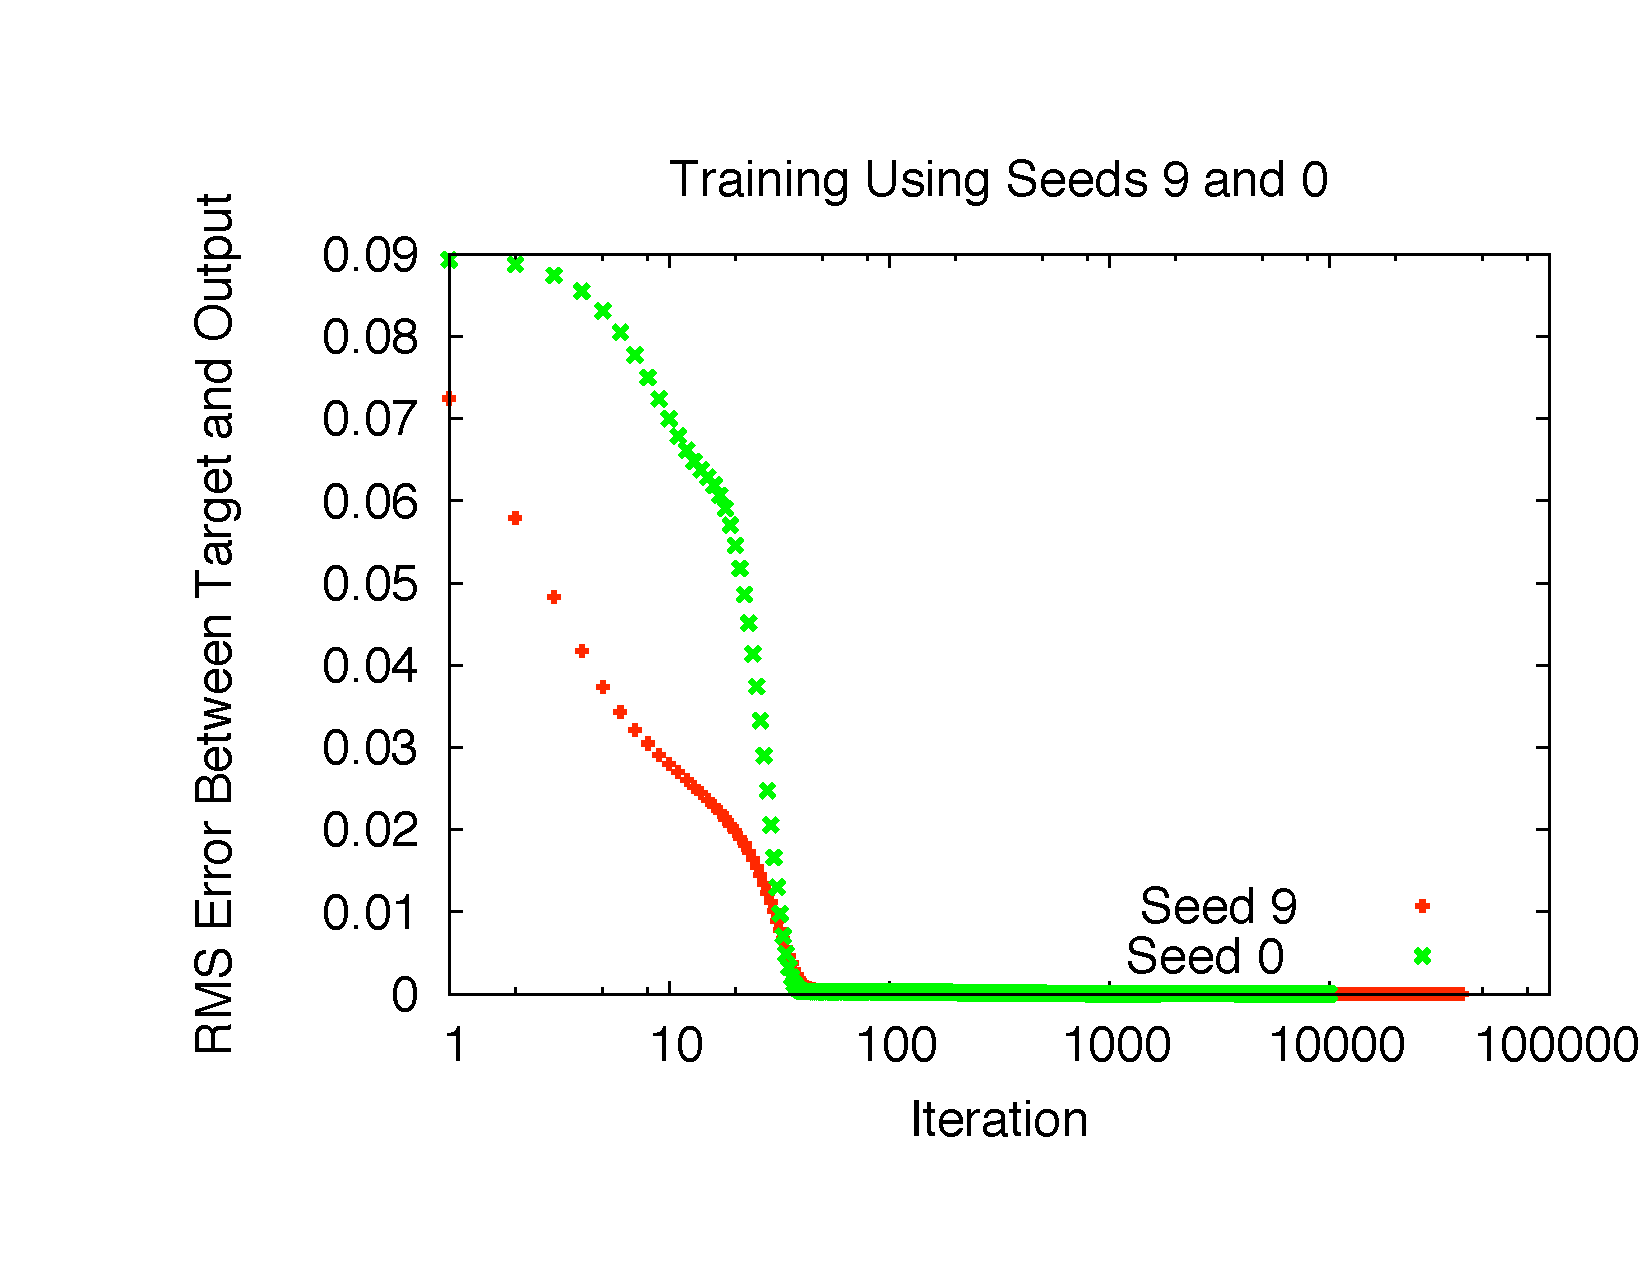
\includegraphics[width=0.85\columnwidth]{../bpgt-3.0/damping_test/Trainings.pdf}
	\caption{Training session comparison for seeds $0$ and $9$. We observe that seed $0$ reaches a local minimum before it completes all iterations}
	\label{fig:bpgt-3.0_damping_test_Trainings}
\end{figure}

Previously, we tested the network with data points that were taught before or that were within the bounds marked by the points the
neural network had been shown. Finally, we test the neural network on a different initial condition. We let $\phi=10$, and by doing so
we expose the neural network to some data it has not encountered before. Furthermore, the data is not within the bounds of data points
that were taught to the neural network. The neural network makes a prediction for the unknown data points when $t > 0.5$. A comparison
between the neural networks prediction and the expected output using equation \ref{eqn:damping} is illustrated in
Figure~\ref{fig:bpgt-3.0_damping_test_output_phi}. Based on this illustration, we observe that the network is capable of making a sane prediction on data points that it has not previously encountered.

\begin{figure}[]
	\centering
	\subfloat[\label{fig:bpgt-3.0_damping_test_output}]{	
			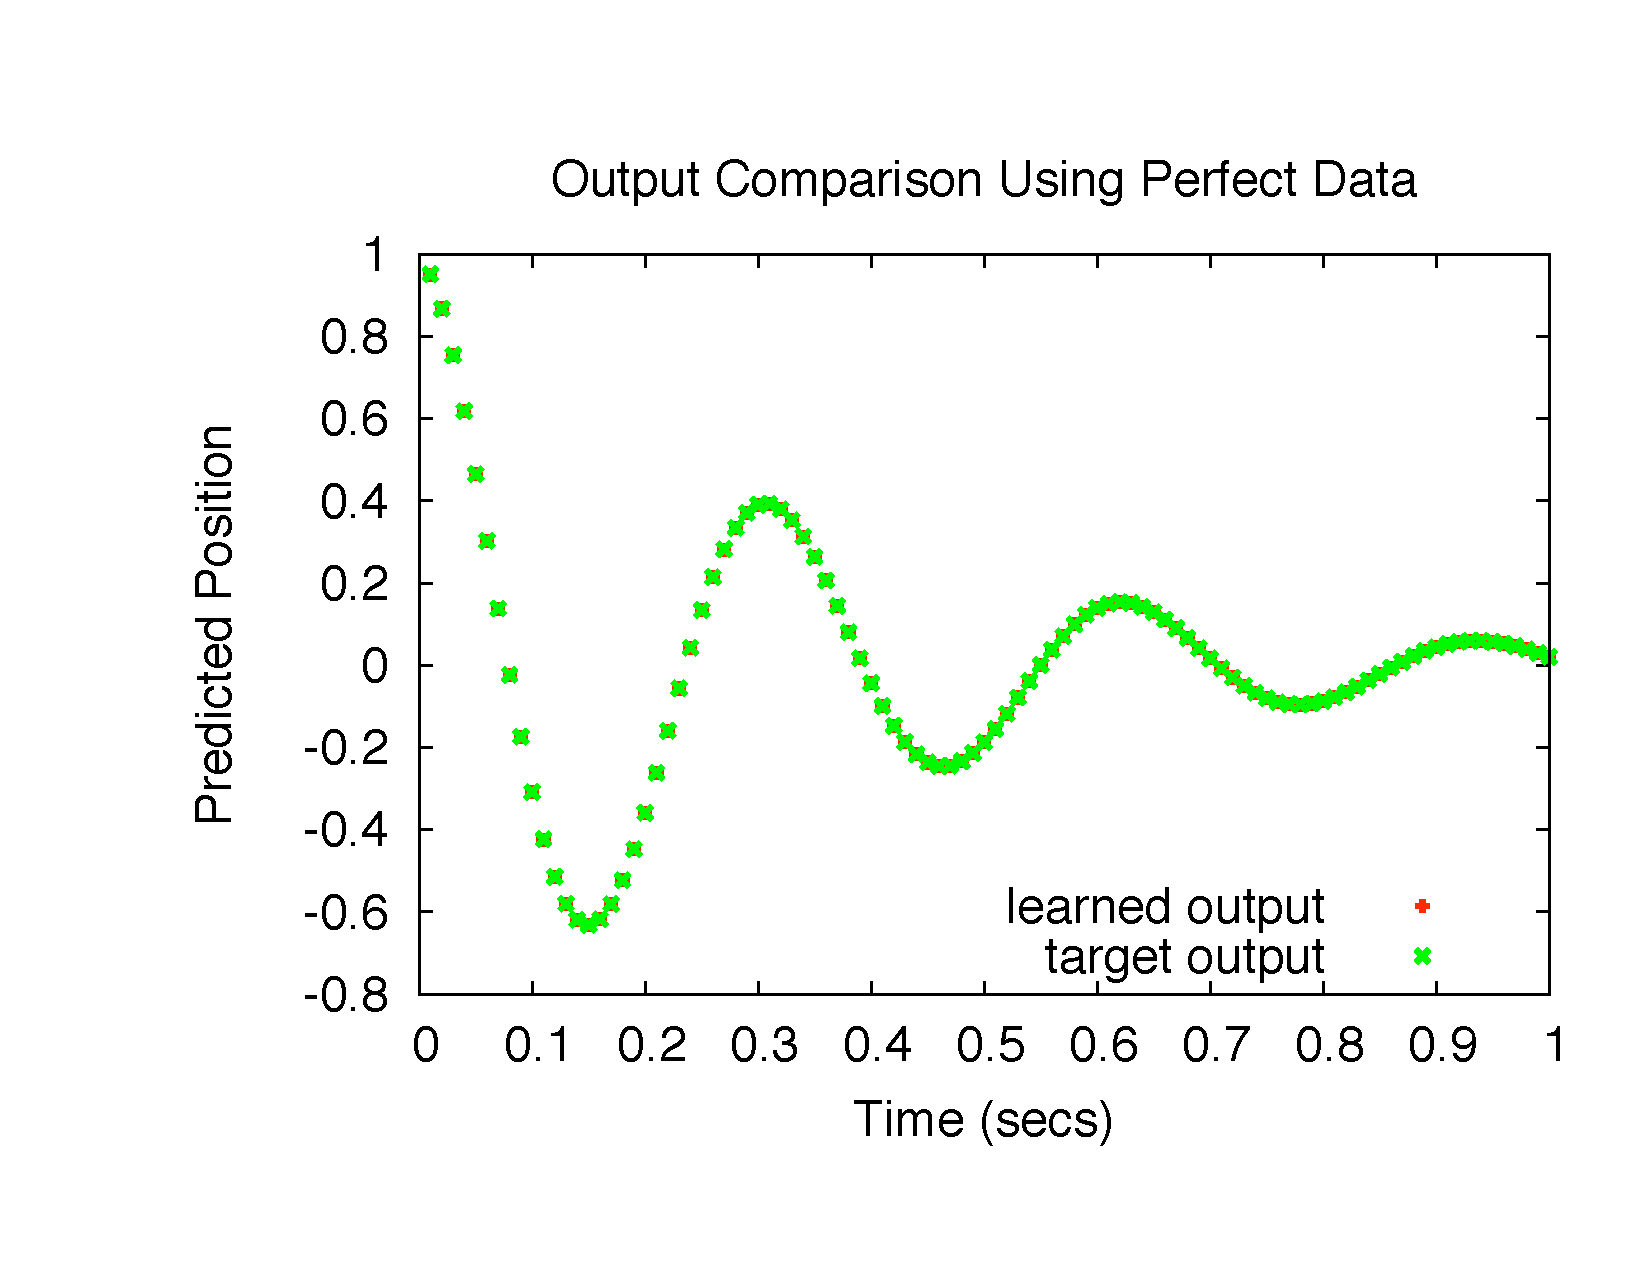
\includegraphics[width=0.49\columnwidth]{../bpgt-3.0/damping_test/output.pdf}
	}
	\subfloat[\label{fig:bpgt-3.0_damping_test_final_output}]{	
			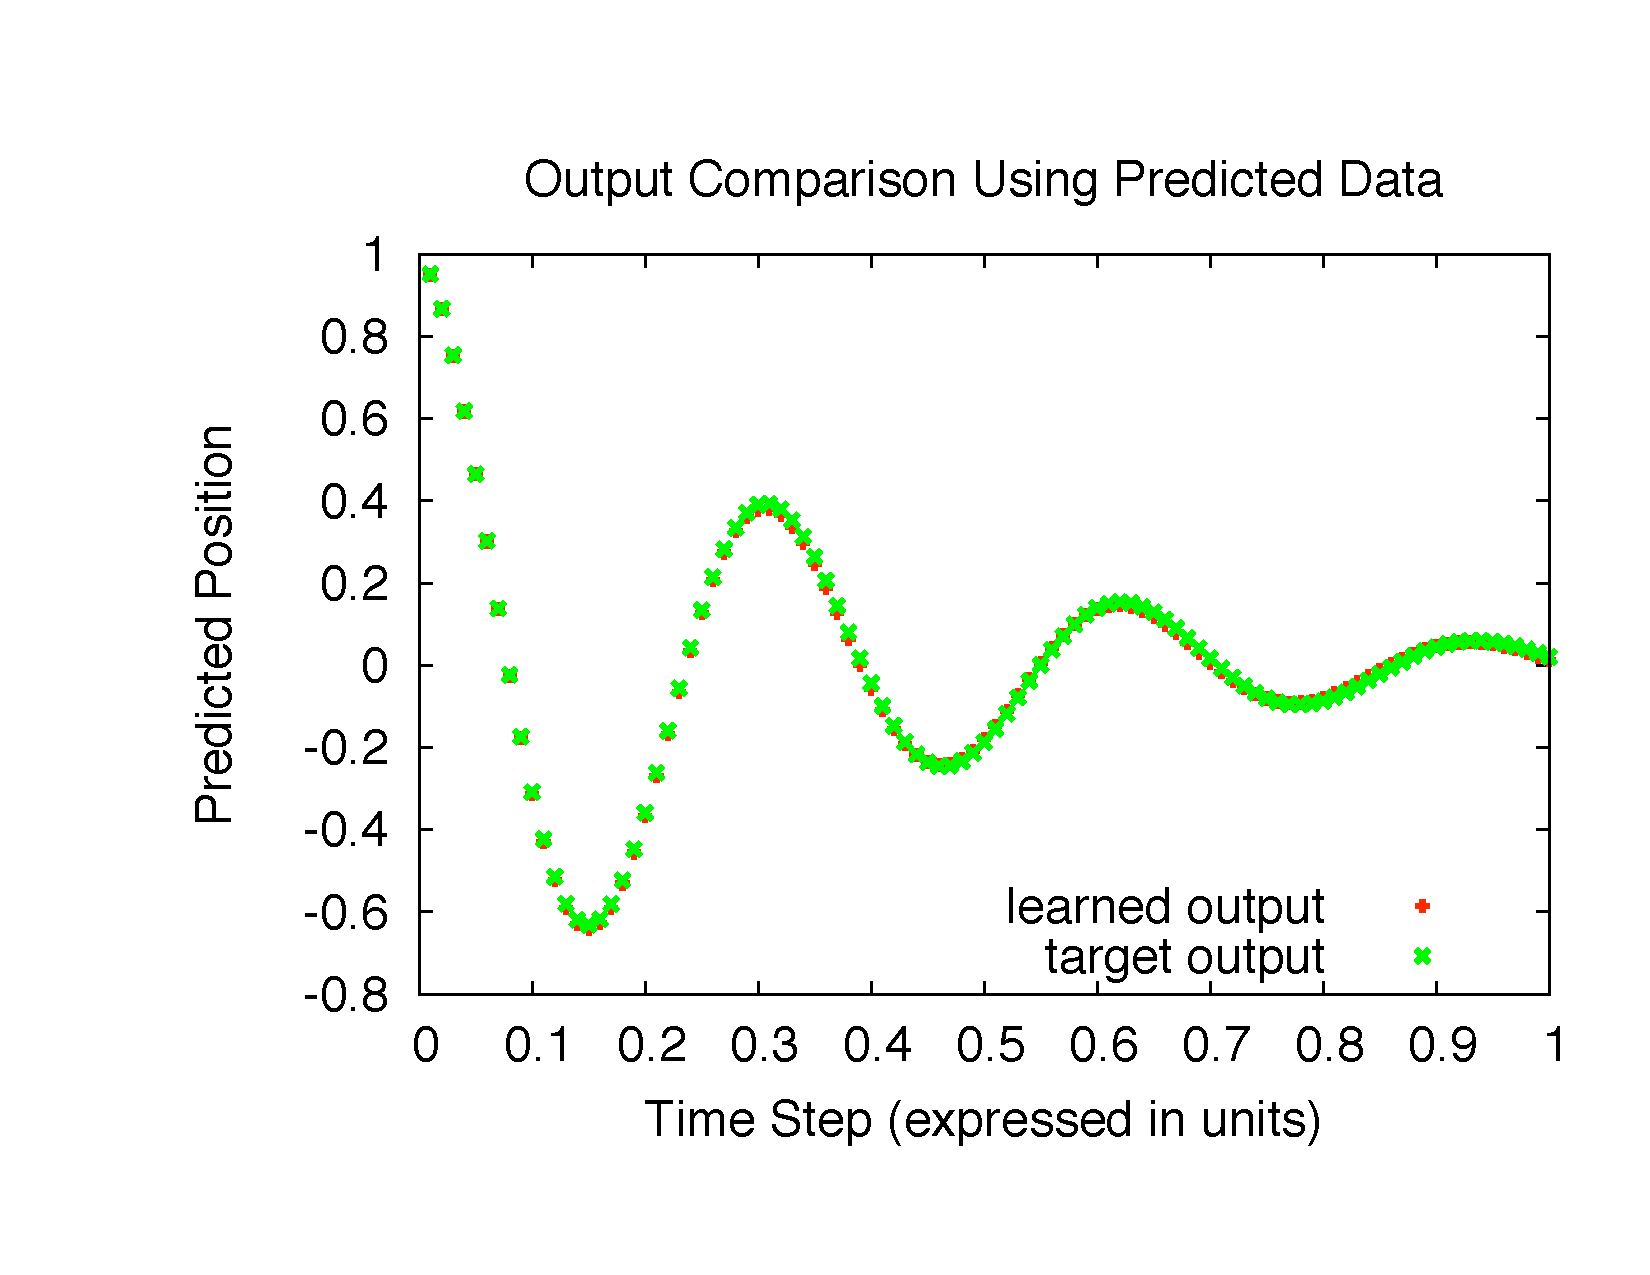
\includegraphics[width=0.49\columnwidth]{../bpgt-3.0/damping_test/final_output.pdf}
	}
		\caption{Output comparison between perfect data (a) and predicted data (b) as input for the neural network. It can be observed in figure (b) that the error is greater and increases as time is increased. Yet, the network can rely on its own generated data relatively well.}
	\label{fig:bpgt-3.0_damping_test_output_comp}	
\end{figure}


\begin{figure}[htbp]
	\centering
		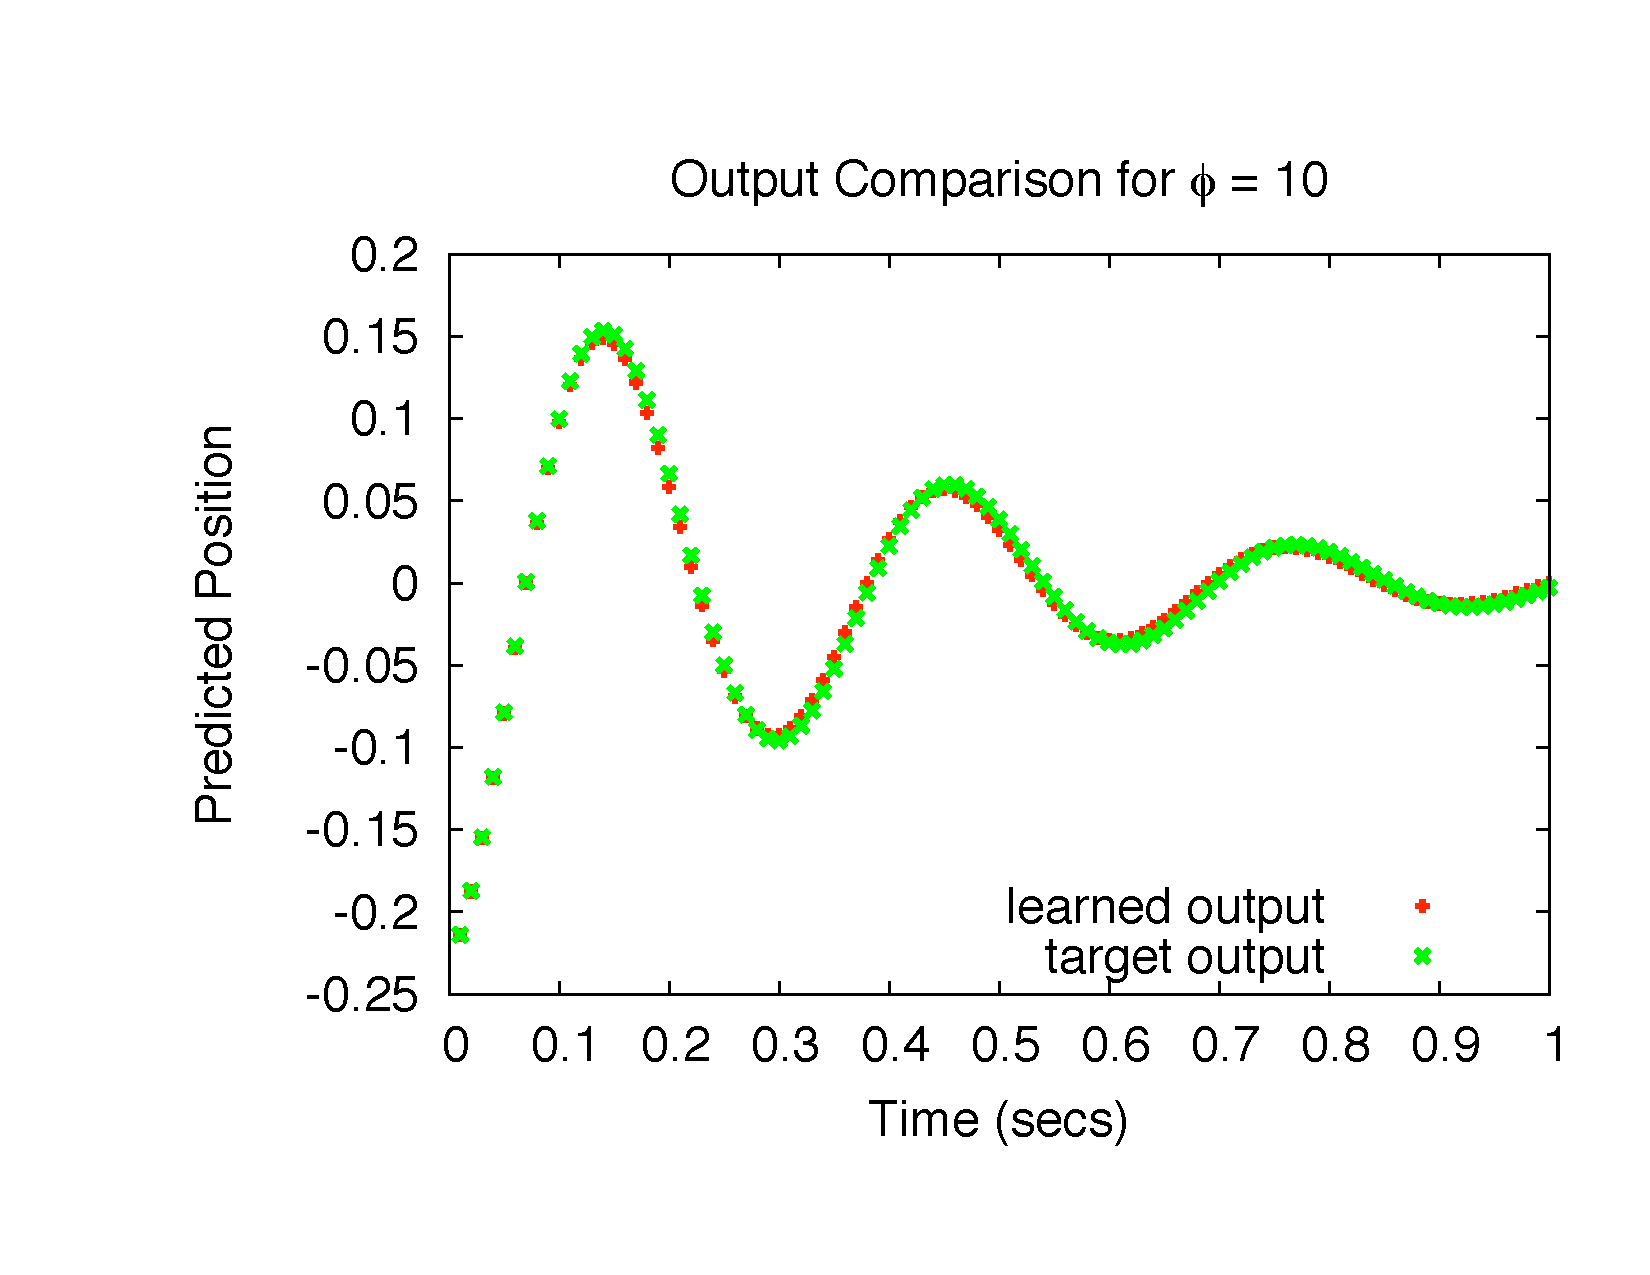
\includegraphics[width=0.85\columnwidth]{../bpgt-3.0/damping_test/output_phi.pdf}
	\caption{Comparison between predicted output and expected output for the neural network when $\phi=10$. Unknown data to the neural network starts when $t > 0.5$}
	\label{fig:bpgt-3.0_damping_test_output_phi}
\end{figure}

% subsection a_more_complex_problem (end)

% section results (end)

\section{Conclusion} % (fold)
\label{sec:conclusion}

The Back-propagation algorithm has time complexity within $O(n)$, which is faster than the RMS Minimization algorithm with a time
complexity of $O(n^{2})$ when varying the number of neurons in the middle layer. 

The Back-propagation algorithm reached a smaller error for the simple examples that the RMS Minimization algorithm.

As observed in some results, the neural network may get stuck in local minima unable to arrive to better solutions. We noticed this in
both the Back-propagation and RMS Minimization algorithms.

The Back-propagation demonstrates in these experiments to be more scalable than the RMS Minimization algorithm in terms of numbers of
neurons in the network. 

The Back-propagation neural network demonstrates ability to solve non-linear problems.

% section conclusion (end)	
\bibliographystyle{plain}
\bibliography{bib/eds}
\end{document} 